\chapter{Results}\label{chap5}
In this section we present the preliminary results of the performance of the $\tauh$ identification algorithm using $\int\mathcal{L} dt=139.2$ fb$^{-1}$ of data recorded between 2015 and 2018.
The correction factors are applied to simulation in order to match the efficiency observed in data. These correction factors are defined as the ratio between the efficiency measured in data and in simulation.
\begin{equation}
C_{\text{ID}}=\frac{\mathcal{E}_{\text{Data}}}{\mathcal{E}_{\text{MC}}}.
\end{equation}
For this work, we present a preview of the value of the correction factors for \textit{Tight} ID working point for $\tauh$ candidates with $\pt$ above 45 GeV. Since this report is about a work in progress and we have not studied yet the effect of the systematic uncertainties on our results, we will take another approach on estimating the correction factors.

\section{Systematic uncertainties}
The values for the systematic uncertainties used to report the value of the correction factors are presented in Table \ref{Tab5}. These numbers have been provided by Terry Wyatt and Sam Dysch, based on their previous experience working on analysis that make use of $Z\to\tauh l$ events.
\begin{table}[H]
	\centering
	\begin{tabular}{cc}
		\hline
		\multicolumn{1}{|c|}{Source}        & \multicolumn{1}{c|}{Sys. Uncertainty (\%)} \\ \hline
		Electron ID efficiency              & 0.8                                        \\
		Muon ID Efficiency                  & 0.2                                        \\
		Electron $\pt$ scale and resolution & 0.4                                        \\
		Muon $\pt$ scale and resolution     & 0.3                                        \\
		Tau $\pt$ scale                     & 1.9                                        \\
		Electron trigger efficiency         & 0.1                                        \\
		Muon trigger efficiency             & 0.4                                        \\ 
		Integrated luminosity               & 1.7                                        \\ \hline
	\end{tabular}
	\caption{Systematic uncertainties used in this study.}
	\label{Tab5}
\end{table}
\section{$\mu\tau$ Final state}
We define the simulation correction factor as
\begin{equation}
	C_{\text{Tight-ID}}=\frac{N_{\text{MC}}}{N_{\text{DATA}}}.
\end{equation}
Where N is the total number of events that pass our selection. The number of events that gets selected after all the cuts and without the $\pt(\tauh)>45$ GeV requirement are shown in Table \ref{Table6}.
\begin{table}[H]
	\centering
	\resizebox{\columnwidth}{!}{%
	\begin{tabular}{ccc}
		\hline
		\multicolumn{1}{c|}{Samples} & \multicolumn{1}{c|}{Before $\pt(\tauh)$\textgreater{}45 GeV cut} & After all cuts      \\ \hline
		Z$\to\tau\tau$               & 34224.49$\pm$420.83(stat)$\pm$581.81(lumi)$\pm$675.88(sys)                                              & 11899.10$\pm$182.66(stat)$\pm$202.28(lumi)$\pm$234.99(sys) \\
		Z+jets                       & 543.21$\pm$11.06(stat)$\pm$9.23(lumi)$\pm$10.73(sys)                                                 & 98.92$\pm$4.69(stat)$\pm$1.68(lumi)$\pm$1.95(sys)      \\
		W+jets                       & 586.70$\pm$77.99(stat)$\pm$9.97(lumi)$\pm$11.59(sys)                                                 & 37.11$\pm$18.75(stat)$\pm$0.63(lumi)$\pm$0.73(sys)     \\
		ttbar                        & 339.94$\pm$6.84(stat)$\pm$5.78(lumi)$\pm$6.70(sys)                                                  & 88.44$\pm$3.42(stat)$\pm$1.50(lumi)$\pm$1.75(sys)      \\
		Diboson                      & 470.69$\pm$4.72(stat)$\pm$8.00(lumi)$\pm$9.30(sys)                                                  & 187.07$\pm$2.82(stat)$\pm$3.18(lumi)$\pm$3.69(sys)     \\
		Single top                   & 63.03$\pm$3.07(stat)$\pm$1.07(lumi)$\pm$1.24(sys)                                                   & 14.35$\pm$1.50(stat)$\pm$0.24(lumi)$\pm$0.28(sys)      \\
		MJ                           & 2386.06$\pm$143.76(stat)$\pm$40.56(lumi)$\pm$47.12(sys)                                               & 231.43$\pm$75.25(stat)$\pm$3.93(lumi)$\pm$4.57(sys)    \\ \hline
		\multicolumn{1}{c|}{MC Total}   & \multicolumn{1}{c|}{38634.12$\pm$668.27(stat)$\pm$656.78(lumi)$\pm$762.96(sys)}                         & 12556.42$\pm$289.09(stat)$\pm$213.46(lumi)$\pm$247.97(sys) \\ \hline
		\multicolumn{1}{c|}{Data}    & \multicolumn{1}{c|}{39101$\pm$198(stat)$\pm$665(lumi)$\pm$772(sys)}                               & 12692$\pm$112(stat)$\pm$216(lumi)$\pm$251(sys)      \\ \hline
	\end{tabular}
	}
	\caption{Number of selected events in data and each of the simulation samples in the $Z\to\tauh\mu$. Statistical and systematica uncertainties are presented separately. Luminosity uncertainty is presented apart.}
	\label{Table6}
\end{table}
The value obtained for $C_{\text{Tight-ID}}$ in the final state that contains one muon and a $\tauh$ candidate is
\begin{equation}
C_{\text{Tight-ID}}=0.989\pm 0.012\text{(stat)}\pm 0.024\text{(lumi)}\pm 0.028\text{(sys)}.
\end{equation}
All the distributions of the relevant cuts for selecting our signal events after applying all the other cuts are shown in Fig.\ref{Fig17} (Appendix A).
\section{$e\tau$ Final state}
For the final state that contains one electron and a $\tauh$ candidate, the number of events that gets selected after all the cuts and without the $\pt(\tauh)>45$ GeV requirement are shown in Table \ref{Table8}.
\begin{table}[H]
	\centering
	\resizebox{\columnwidth}{!}{%
	\begin{tabular}{ccc}
		\hline
		\multicolumn{1}{c|}{Samples} & \multicolumn{1}{c|}{Before $\pt(\tauh)$\textgreater{}45 GeV cut} & After all cuts     \\ \hline
		Z$\to\tau\tau$               & 25269.30$\pm$362.92(stat)$\pm$429.58(lumi)$\pm$531.26(sys)                                              & 8787.97$\pm$150.77(stat)$\pm$149.39(lumi)$\pm$184.76(sys) \\
		Z+jets                       & 682.15$\pm$12.69(stat)$\pm$11.60(lumi)$\pm$14.34(sys)                                                 & 74.07$\pm$4.23(stat)$\pm$1.26(lumi)$\pm$1.56(sys)     \\
		W+jets                       & 348.28$\pm$56.10(stat)$\pm$5.92(lumi)$\pm$7.32(sys)                                                 & 8.08$\pm$8.08(stat)$\pm$0.14(lumi)$\pm$0.17(sys)      \\
		ttbar                        & 255.55$\pm$6.05(stat)$\pm$4.34(lumi)$\pm$5.37(sys)                                                  & 56.63$\pm$2.86(stat)$\pm$0.96(lumi)$\pm$1.19(sys)     \\
		Diboson                      & 384.25$\pm$4.19(stat)$\pm$6.53(lumi)$\pm$8.08(sys)                                                  & 152.92$\pm$2.58(stat)$\pm$2.60(lumi)$\pm$3.21(sys)    \\
		Single top                   & 47.48$\pm$2.71(stat)$\pm$0.81(lumi)$\pm$1.00(sys)                                                   & 11.29$\pm$1.32(stat)$\pm$0.19(lumi)$\pm$0.24(sys)     \\
		MJ                           & 1530.54$\pm$101.21(stat)$\pm$26.02(lumi)$\pm$32.18(sys)                                               & 229.34$\pm$65.04(stat)$\pm$3.90(lumi)$\pm$4.82(sys)   \\ \hline
		\multicolumn{1}{c|}{Total}   & \multicolumn{1}{c|}{28487.55$\pm$545.87(stat)$\pm$484.29(lumi)$\pm$598.91(sys)}                         & 9320.31$\pm$234.87(stat)$\pm$158.44(lumi)$\pm$195.95(sys) \\ \hline
		\multicolumn{1}{c|}{Data}    & \multicolumn{1}{c|}{29723$\pm$172(stat)$\pm$505(lumi)$\pm$625(sys)}                               & 9559$\pm$98(stat)$\pm$162(lumi)$\pm$201(sys)        \\ \hline
	\end{tabular}
	}
	\caption{Number of selected events in data and each of the simulation samples in the $Z\to\tauh e$. Statistical and systematica uncertainties are presented separately. Luminosity uncertainty is presented apart.}
	\label{Table8}
\end{table}
The value obtained for $C_{\text{Tight-ID}}$ is
\begin{equation}
C_{\text{Tight-ID}}=0.975\pm 0.014\text{(stat)}\pm 0.023\text{(lumi)}\pm 0.029\text{(sys)}.
\end{equation}
All the distributions of the relevant cuts for selecting our signal events after applying all the other cuts are shown in Fig.\ref{Fig18} (Appendix A).
\section{Discussion}
As this study makes use of events highly boosted on the transverse plane the Z$(\pt)$ modelling is very important. In the first stages of our analysis we used Powheg+Pythia8 to simulate $Z\to\tauh l$ events. Fig.\ref{Fig23} shows the Z$(\pt)$ and $\Delta\phi(\tauh,l)$ for the muon-tau final state for in-between events. As it can be seen the tendency in the MC is to underestimate the data for high-Z$(\pt)$ values. These results have been previously reported by ATLAS studies \cite{Aad:2019wmn}, and Fig.\ref{Fig20} shows the Z$(\pt)$ modelling made by different generators. This has motivated us to use Sherpa to simulate our signal events. The Z$(\pt)$ results for this generator are shown in Fig.\ref{Fig19} and there is improvement for high-$\pt$ values over Powheg+Pythia8. The complete set of plots showing the Z$(\pt)$ distribution for both e-tau and mu-tau final states for the two different type of topologies are shown in Fig.\ref{Fig21} and Fig.\ref{Fig22}.
\begin{figure}[H]
	\centering
	\subfloat[]{\label{Fig23a}{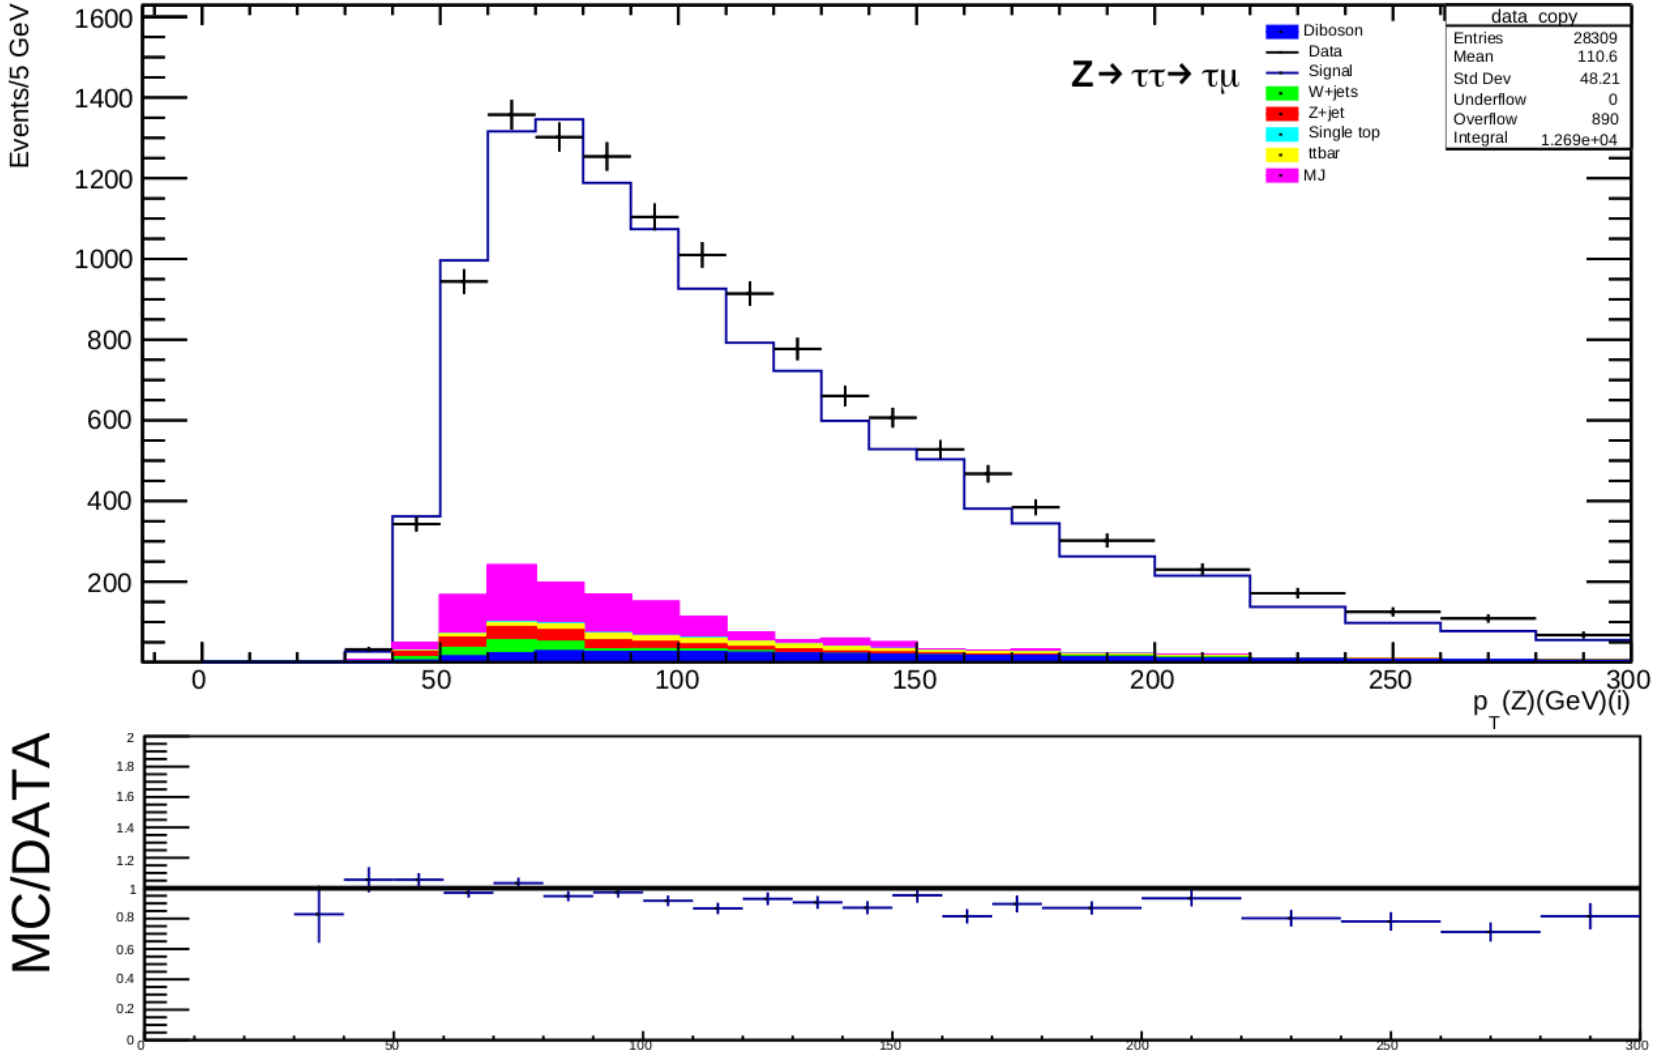
\includegraphics[width=0.50\textwidth]{figures/Fig23a}}}\hfill
	\subfloat[]{\label{Fig23b}{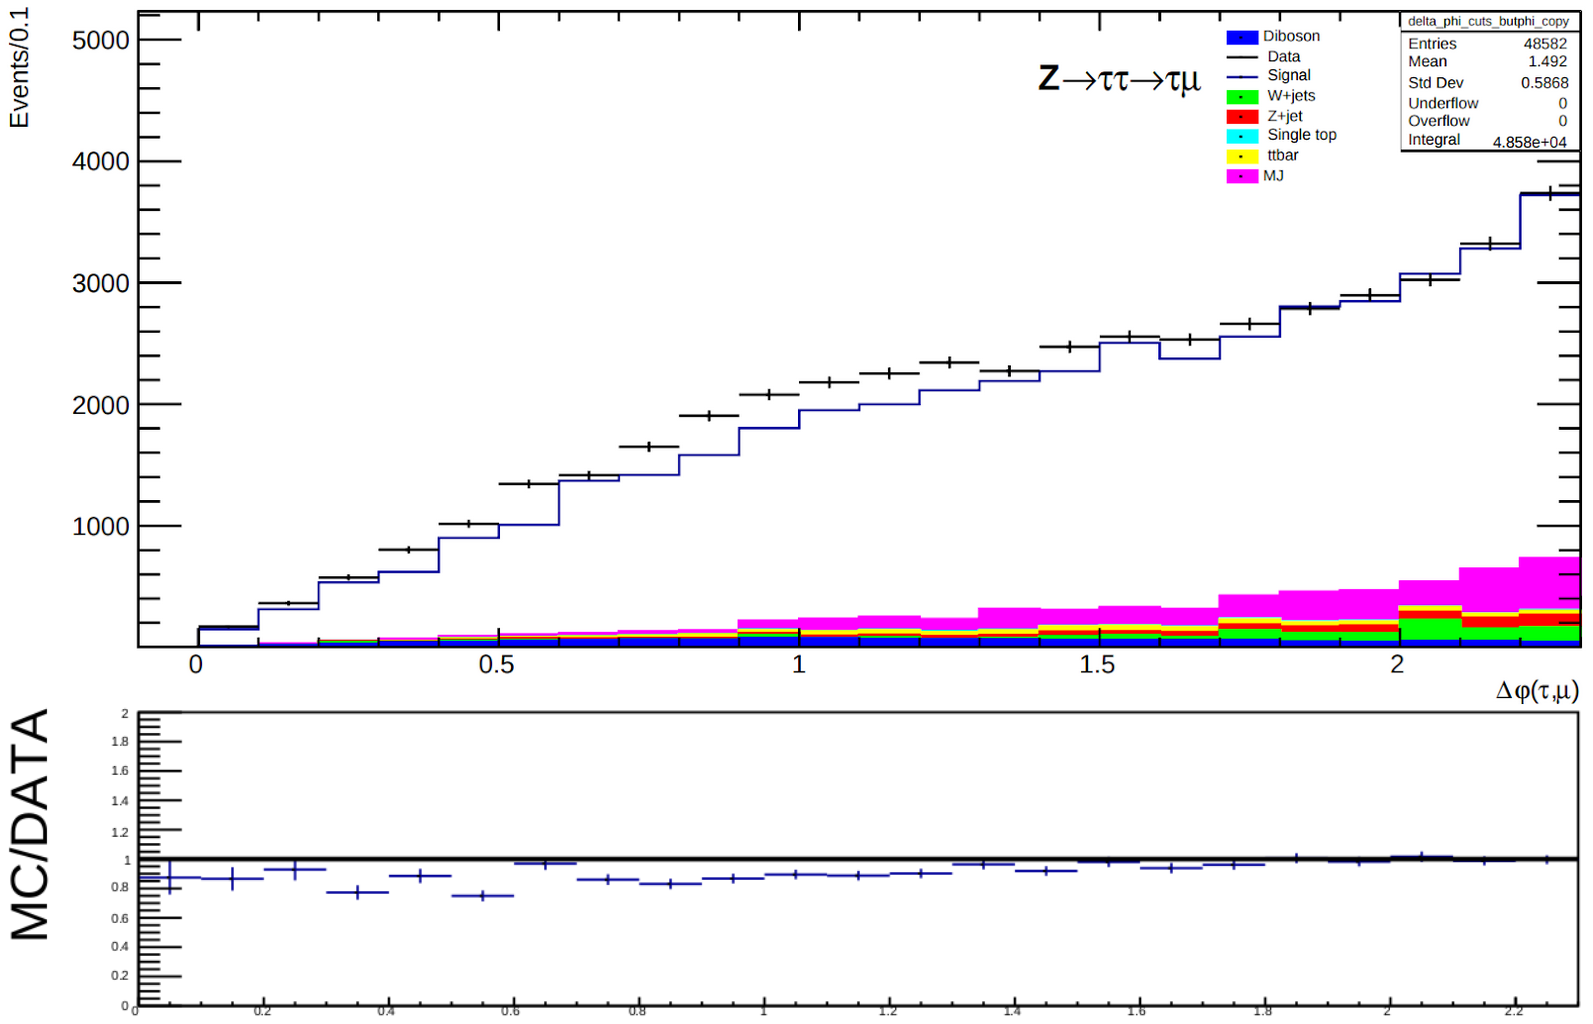
\includegraphics[width=0.50\textwidth]{figures/Fig23b}}}
	\caption{Distribution of Z$(\pt)$ for in-between events (a) and $\Delta\phi(\tauh,l)$ (b) using Powheg+Pythia8. All the other cuts have been applied apart from the one being plotted.}
	\label{Fig23}
\end{figure}
\begin{figure}[H]
	\centering
	\subfloat[]{\label{Fig19a}{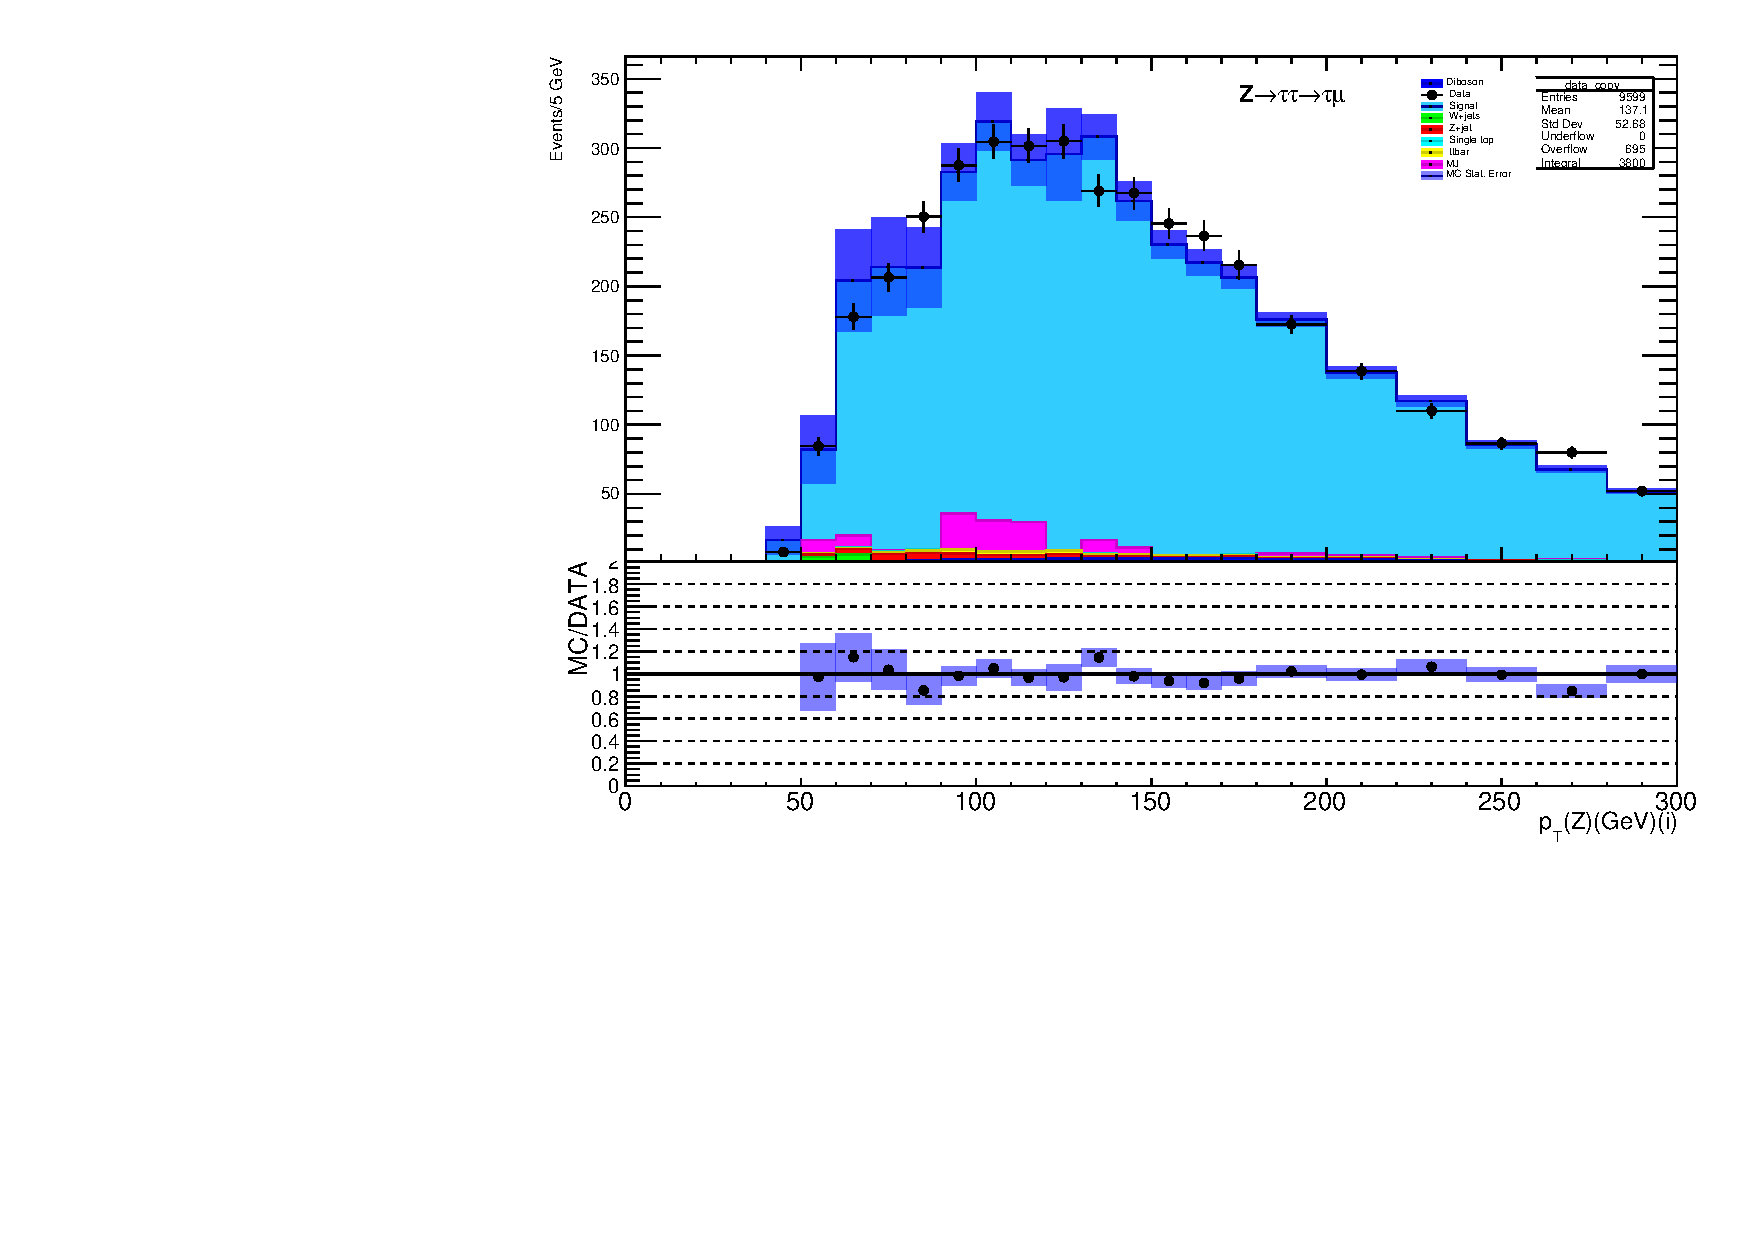
\includegraphics[width=0.50\textwidth]{figures/Fig19a}}}\hfill
	\subfloat[]{\label{Fig19b}{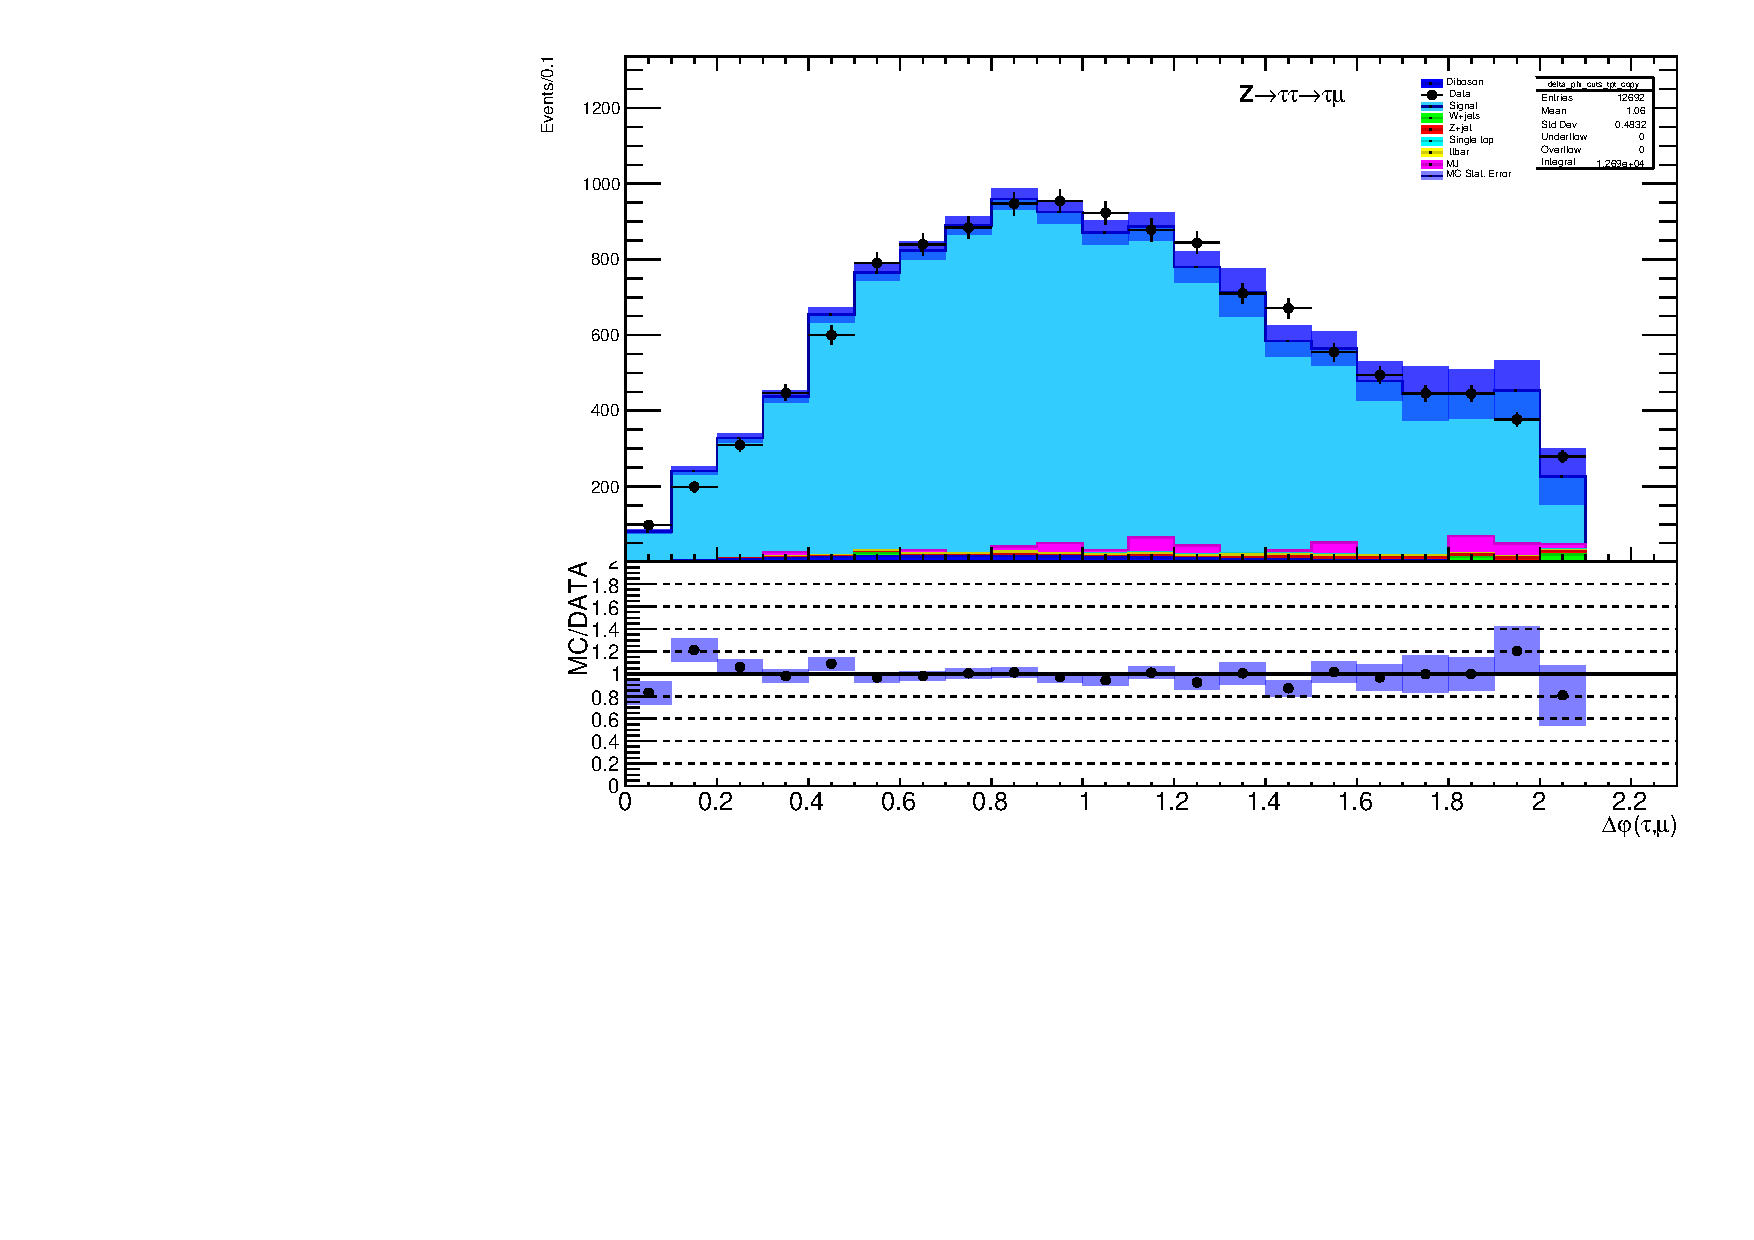
\includegraphics[width=0.50\textwidth]{figures/Fig19b}}}
	\caption{Distribution of Z$(\pt)$ for in-between events (a) and $\Delta\phi(\tauh,l)$ (b) using Sherpa. All the other cuts have been applied apart from the one being plotted.}
	\label{Fig19}
\end{figure}
\begin{figure}[H]
	\centering
	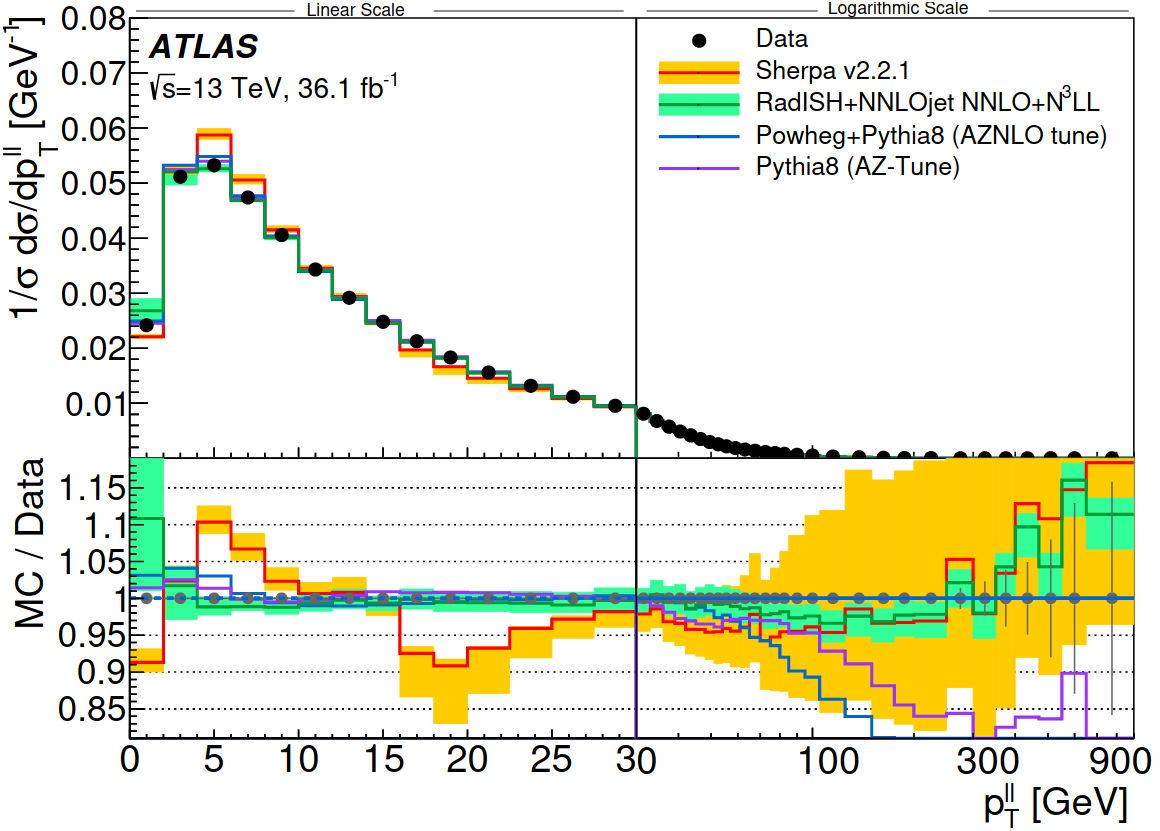
\includegraphics[width=0.5\textwidth]{figures/Fig20}
	\caption{Comparison of the different modelling of the Z$(\pt)$ in Drell-Yan events made by different MC generators. As it can be seen Sherpa does a better job describing the Z boson transverse momentum for higher $(\pt)$ values than Powheg+Pythia8. However both generators underestimate the measured value in the high-Z$(\pt)$ region. Taken from \cite{Aad:2019wmn}.}
	\label{Fig20}
\end{figure}

Another challenging task will be to control the MJ background contribution when we go to looser regions in tau-ID. As it can be seen in Fig.\ref{Fig17c} and Fig.\ref{Fig17d} the MJ background contribution starts to be more important for 1-prong and 3-prong taus for looser values of the RNN score. We have explored the possible correlation that could arise in actual $Z\to\tauh l$ events in variables like the ratio between the transverse momentum of the tau and the lepton or the ratio between the Z$(\pt)$ and the leading jet. The distributions for this variables are shown in Fig.\ref{Fig24a} and Fig.\ref{Fig24b} respectively.
\begin{figure}[H]
	\centering
	\subfloat[]{\label{Fig24a}{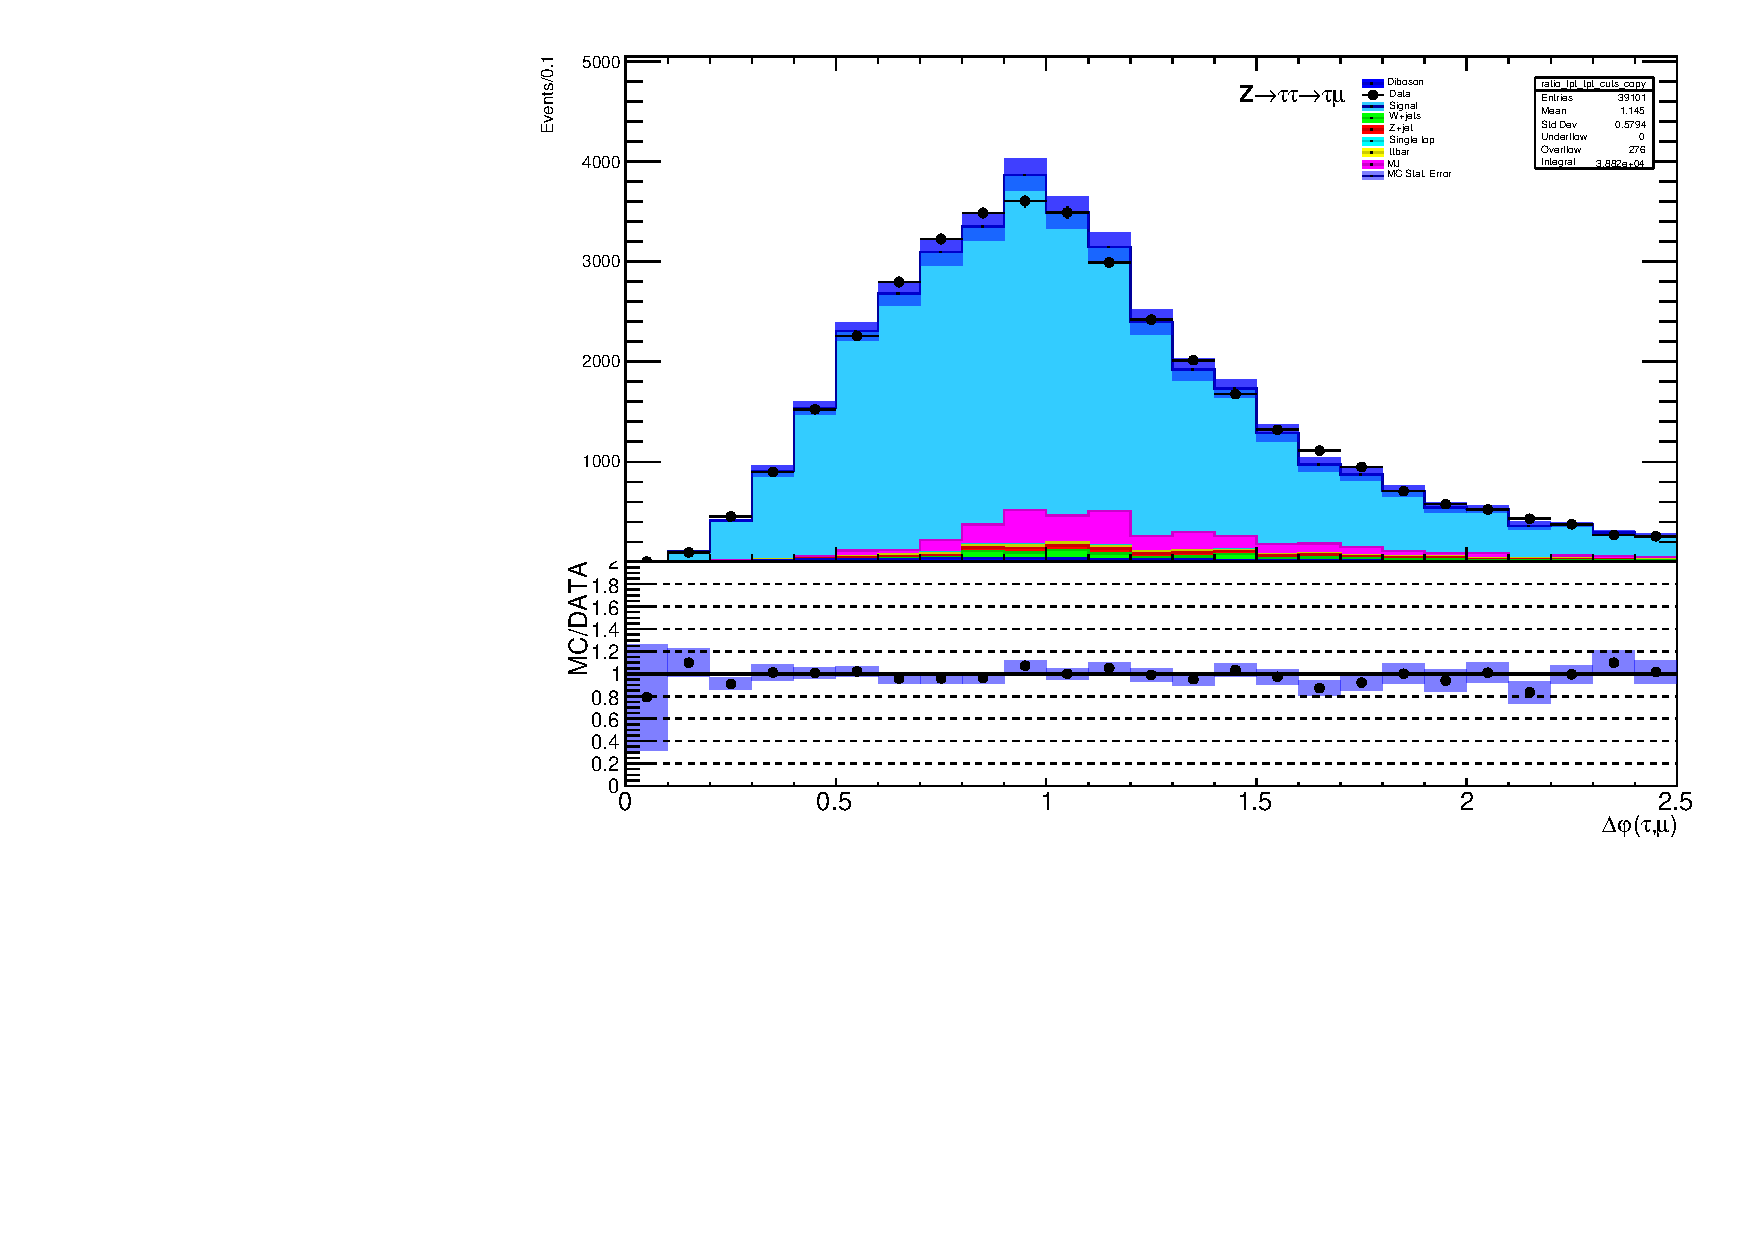
\includegraphics[width=0.50\textwidth]{figures/Fig24a}}}\hfill
	\subfloat[]{\label{Fig24b}{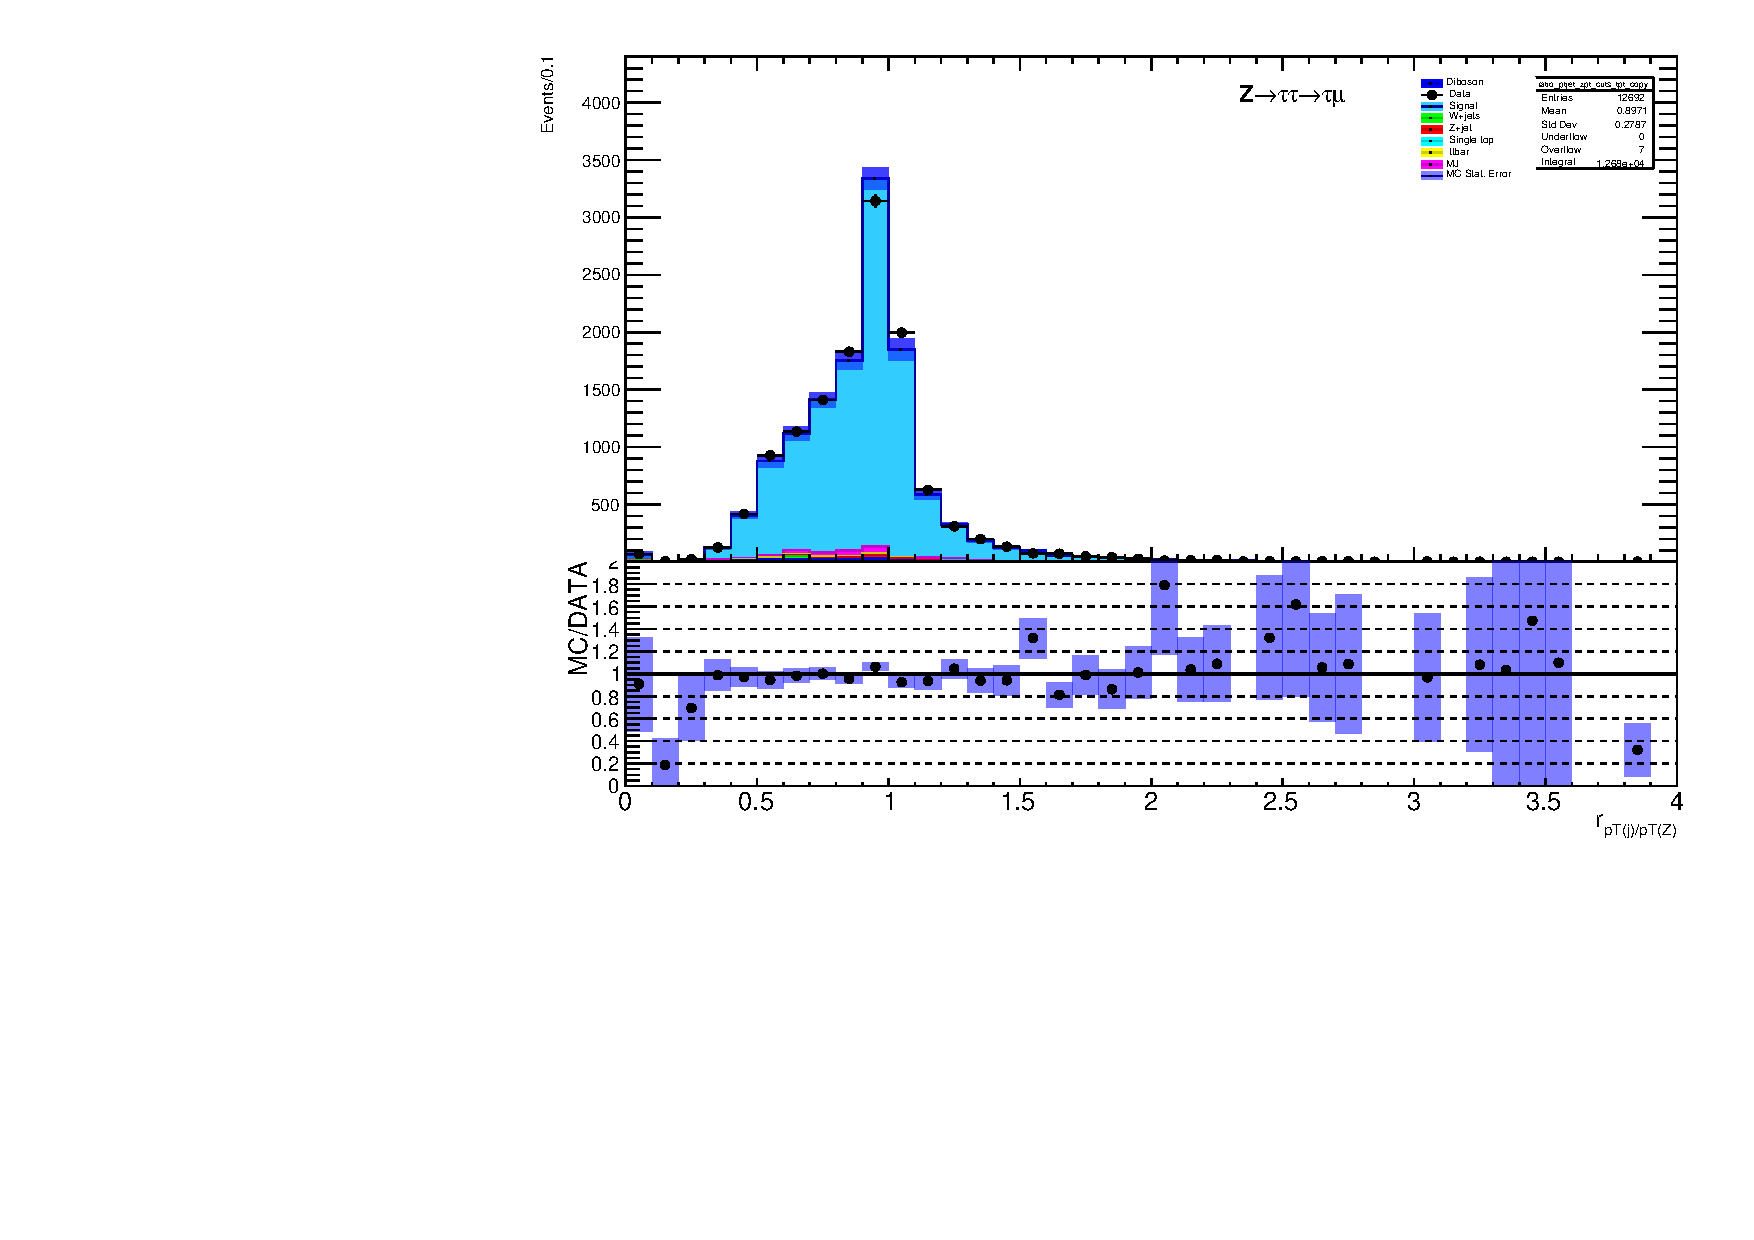
\includegraphics[width=0.50\textwidth]{figures/Fig24b}}}
	\caption{$r_{\frac{\pt(\mu)}{\pt(\tau)}}$ (a) and $r_{\frac{\pt(j)}{\pt(Z)}}$ distributions (b) do not seem to offer a big discriminating power against MJ background events. }
	\label{Fig24}
\end{figure}
These variables though do not offer a discriminating power against the MJ background. 